\documentclass[12pt,a4paper,austrian]{article}
\usepackage{graphicx}
\usepackage[austrian, english]{babel}
\usepackage[utf8]{inputenc}
%\usepackage{listings}
\usepackage{multirow}
\usepackage{epstopdf}
\usepackage{amsmath}
\usepackage{amssymb}
\usepackage{hyperref} % fuer Mengen \N, Q, C, R
\graphicspath{{./fig/}}


%% Satzspiegel
\setlength{\hoffset}{-1in} \setlength{\textwidth}{18cm}
\setlength{\oddsidemargin}{1.5cm}
\setlength{\evensidemargin}{1.5cm}
\setlength{\marginparsep}{0.7em}
\setlength{\marginparwidth}{0.5cm}

\setlength{\voffset}{-1.9in}
\setlength{\headheight}{12pt}
\setlength{\topmargin}{2.6cm}
\addtolength{\topmargin}{-\headheight}
\setlength{\headsep}{3.5cm}
\addtolength{\headsep}{-\topmargin}
\addtolength{\headsep}{-\headheight}
\setlength{\textheight}{27cm}

%% How should floats be treated?
\setlength{\floatsep}{12 pt plus 0 pt minus 8 pt}
\setlength{\textfloatsep}{12 pt plus 0pt minus 8 pt}
\setlength{\intextsep}{12 pt plus 0pt minus 8 pt}

\tolerance2000
\emergencystretch20pt

%% Text appearence
% English text
\newcommand{\eg}[1]%
{\selectlanguage{english}\textit{#1}\selectlanguage{austrian}}

\newcommand{\filename}[1]
{\begin{small}\texttt{#1}\end{small}}

\newcommand\IFT{\unitlength1mm\begin{picture}(10,2) \put (1,1)
{\circle{1.7}} \put(2,1){\line(1,0){5}} \put(8,1)
{\circle*{1.7}}\end{picture}}
\newcommand\FT{\unitlength1mm\begin{picture}(10,2) \put (1,1)
{\circle*{1.7}} \put(2,1){\line(1,0){5}} \put(8,1)
{\circle{1.7}}\end{picture}}

% A box for multiple choice problems
\newcommand{\choicebox}{\fbox{\rule{0pt}{0.5ex}\rule{0.5ex}{0pt}}}

\newenvironment{wahrfalsch}%
{\bigskip\par\noindent\makebox[1cm][c]{richtig}\hspace{3mm}\makebox[1cm][c]{falsch}
    \begin{list}%
    {\makebox[1cm][c]{\choicebox}\hspace{3mm}\makebox[1cm][c]{\choicebox}}%
    {\setlength{\labelwidth}{2.31 cm}\setlength{\labelsep}{3mm}
    \setlength{\leftmargin}{2.61 cm}\setlength{\listparindent}{0pt}
    \setlength{\itemindent}{0pt}}%
    }
    {\end{list}}

\newcounter{theaufgabe}\setcounter{theaufgabe}{1}
\newenvironment{aufgabe}[1]%
{\bigskip\par\noindent\begin{nopagebreak}
                          \textsf{\textbf{\arabic{theaufgabe}.\thinspace Aufgabe}}\quad
                          \textsf{\textit{#1}}\\*[1ex]%
                          \stepcounter{theaufgabe}\hspace{2ex}
\end{nopagebreak}}
{\par\pagebreak[2]}

% Innerhalb der Aufgaben erfolgt die weitere Unterteilung mittels einer
% enumerate Umgebung, die allerdings a), b),... zaehlen soll.
\renewcommand{\labelenumi}{\alph{enumi})}
\renewcommand{\labelenumii}{\arabic{enumii})}

% A box to tick for everything which has to done
\newcommand{\abgabe}{\marginpar{$\Box$}}
% Margin paragraphs on the left side
\reversemarginpar

% Language for listings
%\lstset{language=Vhdl,
%  basicstyle=\small\tt,
% keywordstyle=\tt\bf,
% commentstyle=\sl}

% No indention
\setlength{\parindent}{0.0cm}
% Don't number sections
\setcounter{secnumdepth}{0}


%% Beginning of the text

\begin{document}
    \selectlanguage{austrian}
    \pagestyle{plain}


%===  This is the header section ============================================================
    \thispagestyle{empty}
    \noindent
    \begin{minipage}[b][4cm]{1.0\textwidth}
        \begin{center}
            \begin{bf}
                \begin{large}
                    Digital Signal Processing SS 2024 -- 4.~Assignment
                \end{large} \\
                \vspace{0.3cm}
                \begin{Large}
                    Reconstruction, DFT, FFT, STFT
                \end{Large} \\
                \vspace{0.3cm}
            \end{bf}
            \begin{large}
                Group 22\\
                Julian Feichtinger, K12015812\\
                Wolfram Laube, K08900915\\
            \end{large}
        \end{center}
    \end{minipage}

    \noindent \rule[0.8em]{\textwidth}{0.12mm}\\[-0.5em]
%=======================================================================================


    \begin{aufgabe}{Sampling 1 (40\%)}

        Consider the analog signal

        $$
        x(t)=1+0.5 \cos \left(2 \pi f_{1} t\right)+2 \sin \left(2 \pi f_{2} t\right)+\sin \left(2 \pi f_{3} t\right)
        $$

        with $f_{1}=2 k \mathrm{kz}, f_{2}=4 \mathrm{kHz}$ and $f_{3}=6 \mathrm{kHz}$.

        \begin{enumerate}
            \item[a)] Sketch the Fourier transform of $x(t)$ and plot the analog signal $x(t)$ in Matlab using a timevector $t=0: 1 e-6: 1 e-3$.

            \item[b)]  Sample the analog signal $x(t)$ with sampling frequencies $f_{s 1}=9 \mathrm{kHz}$ and $f_{s 2}=14 \mathrm{kHz}$, which yield $x_{1}[n]$ and $x_{2}[n]$, respectively.
            Sketch the corresponding DTFT spectra.

            \item[c)]  After ideal reconstruction you end up with the analog signals $x_{1}(t)$ and $x_{2}(t)$.
            Sketch the reconstructed analog spectra.
            Plot the reconstructed time-domain signal.
            Compare your results with point a).
        \end{enumerate}

        \hrule
        \begin{enumerate}
            \item[(a)]
\section*{Task (a)}

\subsection*{Problem Statement}
Consider the analog signal
\[ x(t) = 1 + 0.5 \cos \left(2 \pi f_{1} t \right) + 2 \sin \left(2 \pi f_{2} t \right) + \sin \left(2 \pi f_{3} t \right) \]
with \( f_{1} = 2 \, \text{kHz} \), \( f_{2} = 4 \, \text{kHz} \), and \( f_{3} = 6 \, \text{kHz} \).

a) Sketch the Fourier transform of \( x(t) \) and plot the analog signal \( x(t) \) in Python using a time vector \( t = 0:1 \times 10^{-6}:1 \times 10^{-3} \).

\subsection*{Theoretical Background}
The Fourier transform is a mathematical operation that transforms a time-domain signal into its frequency-domain representation. It is crucial for analyzing the frequency components of signals.

Given an analog signal \( x(t) \), its continuous Fourier transform \( X(f) \) is defined as:
\[ X(f) = \int_{-\infty}^{\infty} x(t) e^{-j 2 \pi f t} \, dt \]

For a signal consisting of sinusoids, the Fourier transform will show spikes at the corresponding frequencies.

\subsection*{Mathematical Derivation}
The given signal is:
\[ x(t) = 1 + 0.5 \cos \left(2 \pi f_{1} t \right) + 2 \sin \left(2 \pi f_{2} t \right) + \sin \left(2 \pi f_{3} t \right) \]

The Fourier transform of this signal consists of delta functions at the frequencies of the cosine and sine terms:
\[ X(f) = \delta(f) + 0.25 \left[ \delta(f - f_1) + \delta(f + f_1) \right] - j \left[ \delta(f - f_2) - \delta(f + f_2) \right] - 0.5 j \left[ \delta(f - f_3) - \delta(f + f_3) \right] \]

where:
- The delta function \( \delta(f) \) represents the constant term.
- The cosine term \( 0.5 \cos(2 \pi f_{1} t) \) contributes to delta functions at \( \pm f_1 \).
- The sine terms contribute to delta functions at \( \pm f_2 \) and \( \pm f_3 \), with imaginary coefficients indicating phase shifts.

\subsection*{Python Implementation and Plot}
The plot Figure~\ref{fig:ex1_a_plot} below illustrates the time-domain signal, and Figure~\ref{fig:ex1_a_fft} shows its Fourier transform:

\begin{figure}[h]
    \centering
    \includegraphics[width=0.8\textwidth]{fig/ex1_a_plot.png}
    \caption{Analog Signal $x(t)$}
    \label{fig:ex1_a_plot}
\end{figure}

\begin{figure}[h]
    \centering
    \includegraphics[width=0.8\textwidth]{fig/ex1_a_fft_stem.png}
    \caption{Fourier Transform of $x(t)$}
    \label{fig:ex1_a_fft}
\end{figure}

\subsection*{Conclusion}
The Fourier transform of the given signal shows spikes at the frequencies \( f_1 = 2 \, \text{kHz} \), \( f_2 = 4 \, \text{kHz} \), and \( f_3 = 6 \, \text{kHz} \), corresponding to the cosine and sine terms in the signal. The plot of the analog signal \( x(t) \) illustrates its time-domain behavior over the interval from 0 to 1 ms, and the Fourier transform plot shows the frequency-domain representation with spikes at the expected frequencies.

            %! Author = wolfram_e_laube
%! Date = 06.05.24

\item[(b)]
\section{Task (b): Fourier Transform and Spectrum Visualization}

\subsection{Fourier Transform of $x(t)$}
Given the signal $x(t) = \sin(2\pi 4000 t) + \sin(2\pi 6000 t)$, we calculate the Fourier transform, which reveals delta functions at the frequencies of the sinusoidal components:
$$
X(f) = \frac{1}{2i} \left(\delta(f - 4000) - \delta(f + 4000) + \delta(f - 6000) - \delta(f + 6000)\right)
$$
This expression indicates that the spectrum of $x(t)$ consists of spikes at $\pm 4000$ Hz and $\pm 6000$ Hz.

\subsection{Spectrum Visualization and Sampling Effects}
The spectrum is then visualized, taking into account the sampling frequency $f_s = 10,000$ Hz, which leads to periodic replication of the spectrum. The replication and the combination of these spectra due to sampling are illustrated to show how aliasing could affect the resultant digital signal $x[n]$. The effects are demonstrated using a Python script that plots the original and shifted spectra within the range $-f_s$ to $+f_s$.

\begin{figure}[h]
    \centering
    \includegraphics[width=0.49\textwidth]{fig/ex1_b_plot}
    \caption{Spectrum of \(x(t)\)}
    \label{fig:ex1_b_plot}
\end{figure}

The shifted spectrum plot will show the spectral shifts due to the sampling frequency and illustrate the overlapping spectra.
            %! Author = wolfram_e_laube
%! Date = 06.05.24

\item[(c)]
The Python code accomplishing this is:

\begin{verbatim}
import numpy as np
import matplotlib.pyplot as plt

# Parameters
fs_analog = 100e3  # 100 kHz
fs = 10e3  # 10 kHz
f1 = 4e3  # 4 kHz
f2 = 6e3  # 6 kHz
t_end = 2e-3  # 2 ms

# Time vectors
t = np.arange(0, t_end, 1/fs_analog)
n = np.arange(0, int(t_end * fs))

# Analog signal
x_t = np.sin(2 * np.pi * f1 * t) + np.sin(2 * np.pi * f2 * t)

# Sampled signal
x_n = np.sin(2 * np.pi * f1 * n / fs) + np.sin(2 * np.pi * f2 * n / fs)

# Plotting
plt.figure()
plt.plot(t * 1e3, x_t, label='Analog signal x(t)')
plt.stem(n * 1e3 / fs, x_n, linefmt='r', markerfmt='ro', basefmt=' ', label='Sampled signal x[n]', use_line_collection=True)
plt.xlabel('Time (ms)')
plt.ylabel('Amplitude')
plt.title('Analog and Sampled Signals')
plt.legend()
plt.grid(True)
plt.show()
\end{verbatim}

\begin{figure}[h]
    \centering
    \includegraphics[width=0.49\textwidth]{fig/ex1_c_plot}
    \caption{Analog and Sampled Signals of \(x(t)\)}
    \label{fig:ex1_c_plot}
\end{figure}

        \end{enumerate}

    \end{aufgabe}

    \begin{aufgabe}{Sampling 2 (25\%)}

        100 values of an analog signal $x(t)$ were measured with a sampling time of $1 \mathrm{~ms}$, leading to the discrete-time signal $x[n]$.
        This time domain signal $x[n]$ is transformed to frequency domain using the DFT/FFT, i.e., a 100-point DFT/FFT is calculated.

        \begin{enumerate}
            \item[(a)] What is the frequency spacing between two neighboring spectral points in the DFT spectrum, i.e., what is the frequency resolution?

            \item[(b)] What is the "period" of the DFT spectrum in terms of samples, in terms of frequency, and in terms of normalized angular frequency?

            We now append zeros to the discrete-time signal $x[n]$ to obtain a signal that has a length of 128 samples.

            \item[(c)] Why do we append exactly so many zeros, so that a total signal of length $128=2^{7}$ results?

            \item[(d)] What is the frequency spacing between two neighboring spectral points in the DFT spectrum now?

            \item[(e)] How can the changed distance between two neighboring spectral points be interpreted?
        \end{enumerate}

        \hrule

        \begin{enumerate}
    %        \item[(a)]
\section{Block Diagram of the LTI System}

\subsection*{Problem Statement}
Sketch the block diagram of the LTI system corresponding to the given difference equation:
\[ y[n] = x[n] - \frac{1}{15} y[n-1] + \frac{2}{5} y[n-2] \]

\subsection*{Theoretical Background}
A block diagram for an LTI (Linear Time-Invariant) system visually represents the flow of signals and the operations applied to them. The difference equation can be transformed into a block diagram using delay elements \( z^{-1} \), multipliers, and adders.

\subsection*{Mathematical Derivation}
The given difference equation is:
\[ y[n] = x[n] - \frac{1}{15} y[n-1] + \frac{2}{5} y[n-2] \]

This can be expressed in terms of block diagram components:
\begin{itemize}
    \item \( x[n] \) is the input signal.
    \item \( y[n] \) is the output signal.
    \item \( y[n-1] \) and \( y[n-2] \) are delayed versions of the output signal.
    \item Multipliers \( -\frac{1}{15} \) and \( \frac{2}{5} \) scale the delayed outputs.
    \item An adder combines the scaled delayed outputs with the input signal to produce the output.
\end{itemize}

\subsection*{Block Diagram}
The block diagram representation is as follows:

\begin{figure}[h]
    \centering
    \includegraphics[width=0.8\textwidth]{fig/ex2_a_block_diagram.png}
    \caption{Block Diagram of the LTI System}
    \label{fig:ex2_a_block_diagram}
\end{figure}

\subsection*{Conclusion}
The block diagram illustrates the flow of the input signal \( x[n] \), the delayed outputs \( y[n-1] \) and \( y[n-2] \), and their scaled versions being combined to form the output signal \( y[n] \).

    %        %! Author = wolfram_e_laube
%! Date = 06.05.24

\item[(b)]
\begin{figure}[h]
    \centering
    \includegraphics[width=0.49\textwidth]{fig/ex2_b_plot}
    \caption{Spectrum of \(x(t)\)}
    \label{fig:ex2_b_plot}
\end{figure}

        \end{enumerate}

    \end{aufgabe}

    \begin{aufgabe}{Reconstruction (35\%)}

In image processing, besides other methods, also the FFT can be utilized to conduct edge detection. To this end, a two-dimensional FFT (MATLAB command: $f f t 2$ ) is calculated from an image to transform it from spatial domain to frequency domain. Here, edges in an image produce high frequencies in the corresponding spectrum.

In this exercise, you should make the edges of an image visible. Start by making yourself familiar with the MatLAB script fft_edge_detection. Now filter the image in frequency domain, such that the edges become visible after a transformation back to spatial domain. Describe your approach and justify why it works. A solution could look the one depicted in Fig. 1.
![](https://cdn.mathpix.com/cropped/2024_05_20_fb408b21a3cafdbd1f66g-2.jpg?height=480&width=1612&top_left_y=771&top_left_x=220)

Figure 1 Example for edge detection with the FFT.

        \hrule

        \begin{enumerate}
%            %! Author = wolfram_e_laube
%! Date = 06.05.24

\item[(a)]
The positive frequencies are \( f_0, 2f_0, \ldots, n f_0 \) where \( f_0 = 1 \mathrm{kHz} \).
%            %! Author = wolfram_e_laube
%! Date = 02.04.24

\item [b)]
Plotting the Signals

Figure~\ref{fig:SignalPlot} shows two subplots, one for each frequency. In each subplot, it plots the original signal,
the time-delayed signal (in red dashed lines), and the phase-shifted signal (in green dot-dashed lines,
slightly transparent for better visibility).
The time-delayed and phase-shifted signals are expected to overlap completely,
demonstrating that a time delay is equivalent to a phase shift in the time domain.
\begin{figure}[!ht]
	\centering
	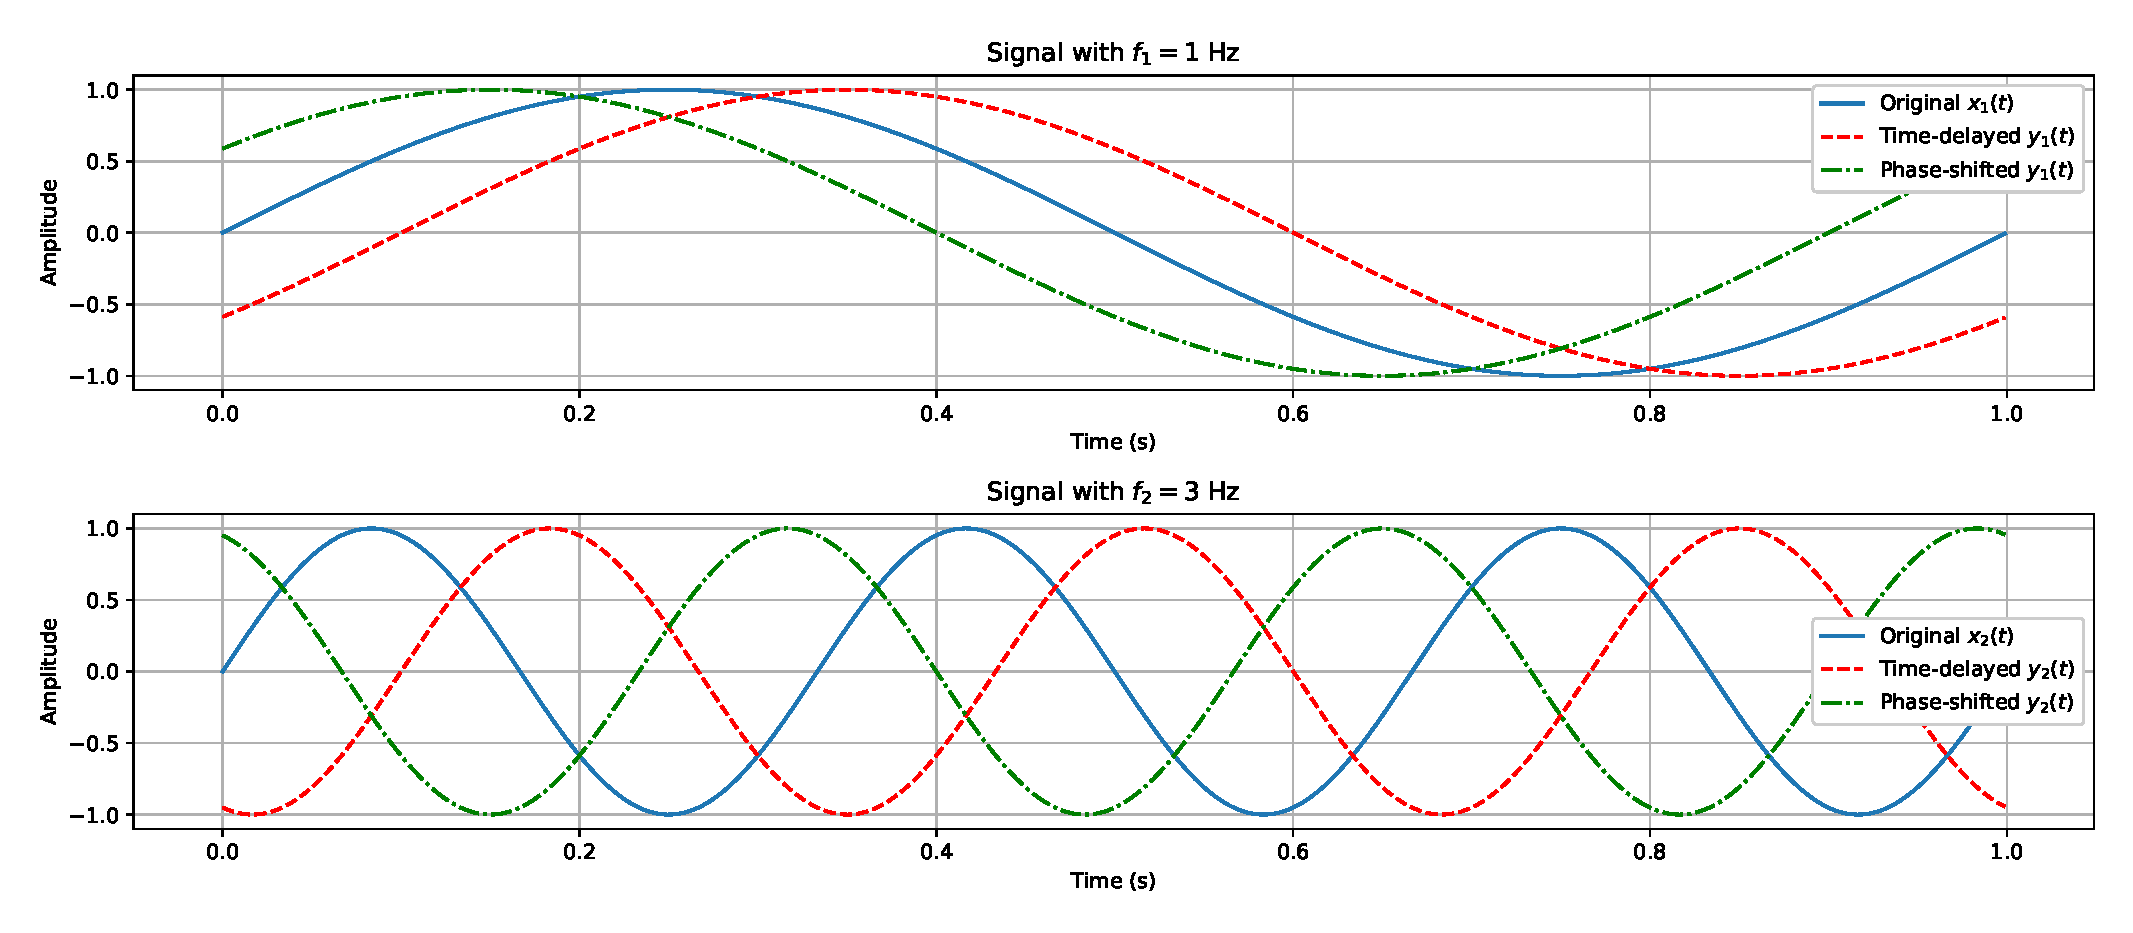
\includegraphics[width=18cm]{ex3_signal_plot.eps}
	\vspace{-0.3cm}
	\caption{Signal Plot.}
	\label{fig:SignalPlot}
	\vspace{-0.1cm}
\end{figure}



%            %! Author = wolfram_e_laube
%! Date = 06.05.24

\item[(c)]
\subsection{Task (c): Qualitative Spectrum Drawing of $x(t)$ up to 20 kHz}

\subsubsection{Problem Statement}
Qualitatively draw the spectrum of the analog signal $x(t)$ up to 20 kHz, considering the effect of zero-order hold (ZOH) reconstruction. Delta pulses should be drawn with an arrow, where the height of the arrow indicates the weight of the delta-pulse.

\subsubsection{Background and Analysis}
\begin{enumerate}
    \item \textbf{Zero-Order Hold (ZOH) Characteristics:}
    The zero-order hold DAC holds each discrete signal value constant over the sample interval, effectively creating a step function between samples. The impulse response of this operation is a rectangular pulse, whose Fourier transform is a sinc function, resulting in a sinc-shaped spectrum that modifies the frequency components of the original signal.

    \item \textbf{Spectral Components:}
    \begin{itemize}
        \item \textbf{Base Frequency:} The original discrete-time signal $x[n]$ has a fundamental frequency of 1000 Hz, resulting in a corresponding delta pulse in the spectrum.
        \item \textbf{Power Calculation:} The power of a sinewave with amplitude $A$ is given by $P = \frac{A^2}{2}$. For $x[n]$, $A = \sqrt{2}$, so $P = 1$ watt, which will be represented by the height of the delta pulse at 1000 Hz.
    \end{itemize}

    \item \textbf{Sinc Function Influence:}
    The frequency response of the ZOH is given by a sinc function, which affects the amplitude of the spectral components. This influence results in a primary lobe around the baseband frequency and side lobes that attenuate in amplitude as they move away from the center frequency.

    \item \textbf{Normalized Sinc:}
    MATLAB and other DSP tools often use a normalized sinc function, which means the function has a maximum of 1 at zero frequency and its first null at the sampling frequency $f_s = 8000$ Hz, serving as a guideline for the drawing.
\end{enumerate}

\subsubsection{Steps for Drawing the Spectrum}
\begin{itemize}
    \item \textbf{Delta Pulse at 1000 Hz:} Mark a delta pulse at 1000 Hz with a height representing the power level of 1 watt.
    \item \textbf{Overlay Sinc Function:} Overlay a sinc function shape across the spectrum. The main lobe should center around 1000 Hz, and side lobes should decrease in amplitude as they extend outwards.
    \item \textbf{Consider Sinc Attenuation:} Show how the sinc function modifies the spectrum, particularly how it attenuates frequencies around 8000 Hz and 16000 Hz just before reaching the nulls.
\end{itemize}

\subsubsection{Conclusion}
The spectrum of $x(t)$ will exhibit characteristics dominated by the sinc function due to the ZOH effect, with a notable delta pulse at the fundamental frequency of 1000 Hz. The qualitative drawing will reflect the sinc function's impact, emphasizing the primary and side lobes up to 20 kHz.

\begin{figure}[h]
    \centering
    \includegraphics[width=0.49\textwidth]{fig/ex3_c_plot}
    \caption{Qualitative Spectrum of \(x(t)\)}
    \label{fig:ex3_c_plot}
\end{figure}

        \end{enumerate}

    \end{aufgabe}

    \begin{aufgabe}{Signal Processing Onramp - BONUS (15\%)}
        This task is optional (additional 15\%) and should help you to learn the basics of practical signal processing techniques in MATLAB.
        You will find out how to use spectral analysis and filtering for preprocessing, analyzing, and extracting information from signal data.

        For that, you need to carry out the full \emph{'Signal Processing Onramp course'}.
        \footnote{\url{https://matlabacademy.mathworks.com/details/signal-processing-onramp/signalprocessing}}
        To get the bonus points, you need to add the certificate to your protocol (you can download a pdf -
        see \emph{'Share Certificate and Progress'}).
        Also, you need to share your progress with my account (\texttt{matthias.wagner@jku.at}),
        which can be done in the same tab.

        \vspace{1em}
        \hrule

%\begin{enumerate}
%        %! Author = wolfram_e_laube
%! Date = 16.04.24

\item[(a)]
A Python function to calculate the DTFT of a finite sequence is provided below.
The function employs NumPy's vectorized operations to avoid explicit for-loops.

\begin{verbatim}
import numpy as np

def dtft(x, n, w):
    """
    Compute the Discrete-time Fourier Transform (DTFT) of a finite sequence.

    :param x: Finite duration sequence over n (numpy array)
    :param n: Sample position vector (numpy array)
    :param w: Frequency location vector (numpy array)
    :return: DTFT values computed at w frequencies (numpy array)
    """
    # Convert all inputs to numpy arrays to ensure proper calculations
    x = np.array(x)
    n = np.array(n)
    w = np.array(w)

    # Create a 2D meshgrid for the frequencies and samples for broadcasting
    N, W = np.meshgrid(n, w)

    # Compute the DTFT using broadcasting and vectorized operations
    X = np.exp(-1j * N * W) @ x
    return X
\end{verbatim}

This function calculates the DTFT using matrix multiplication, which is a vectorized operation
that can replace explicit looping constructs.

%        \item[(b)]
\section*{Task (b)}

\subsection*{Problem Statement}
Compute the spectrum for the whole signal length using the MATLAB command `fft`. Plot the magnitude of the spectrum. Label the axes correctly, with the frequency axis scale in Hz (Hint: the frequency values given in Table 1 should be visible at the correct position on the frequency axis).

\subsection*{Python Script}
\begin{verbatim}
import numpy as np
import matplotlib.pyplot as plt
from scipy.io import wavfile
import os

# Create fig directory if it doesn't exist
if not os.path.exists('fig'):
    os.makedirs('fig')

# Read the DTMF signal from the WAV file
fs, signal = wavfile.read('dtmf.wav')

# Compute the FFT for the whole signal length
spectrum = np.fft.fft(signal)
frequencies = np.fft.fftfreq(len(signal), 1/fs)

# Plot the magnitude spectrum
plt.figure(figsize=(10, 6))
plt.plot(frequencies[:len(frequencies) // 2], np.abs(spectrum[:len(frequencies) // 2]))
plt.title('Magnitude Spectrum of the Entire DTMF Signal')
plt.xlabel('Frequency (Hz)')
plt.ylabel('Magnitude')
plt.grid(True)
plt.savefig('fig/ex4_b_dtmf_spectrum.png')
plt.show()
\end{verbatim}

\subsection*{Magnitude Spectrum of the Entire DTMF Signal}
\begin{figure}[h]
    \centering
    \includegraphics[width=0.8\textwidth]{fig/ex4_b_dtmf_spectrum.png}
    \caption{Magnitude Spectrum of the Entire DTMF Signal}
    \label{fig:ex4_b_dtmf_spectrum}
\end{figure}

\subsection*{Analysis}
The magnitude spectrum of the entire DTMF signal shows the frequencies present in the signal. The frequencies corresponding to the DTMF tones listed in Table 1 should be visible at the correct positions on the frequency axis, confirming the presence of these tones in the signal.

%        %! Author = wolfram_e_laube
%! Date = 16.04.24

\item[(c)]
To observe the impact of varying $\Omega$, the Python code below alters the frequency resolution and compares the results:

\begin{verbatim}
import matplotlib.pyplot as plt
import numpy as np

# Varying the frequency resolution
w_coarse = np.linspace(-np.pi, np.pi, 100)
w_fine = np.linspace(-np.pi, np.pi, 1600)
X_coarse = dtft(x, n, w_coarse)
X_fine = dtft(x, n, w_fine)

# Plot the magnitude response for both resolutions
plt.figure(figsize=(14, 5))
plt.subplot(1, 2, 1)
plt.plot(w_coarse, np.abs(X_coarse))
plt.title('Coarse Frequency Resolution')
plt.xlabel('Frequency (rad/sample)')
plt.ylabel('Magnitude')
plt.grid()

plt.subplot(1, 2, 2)
plt.plot(w_fine, np.abs(X_fine))
plt.title('Fine Frequency Resolution')
plt.xlabel('Frequency (rad/sample)')
plt.ylabel('Magnitude')
plt.grid()

plt.tight_layout()
plt.show()
\end{verbatim}

The DTFT results are calculated and plotted with both coarse and fine frequency resolutions to observe differences in the spectrum.
A finer resolution unveils more details in the frequency domain representation of the signal.

%\end{enumerate}

    \end{aufgabe}


\end{document}
